\documentclass[twoside]{book}

% Packages required by doxygen
\usepackage{fixltx2e}
\usepackage{calc}
\usepackage{doxygen}
\usepackage[export]{adjustbox} % also loads graphicx
\usepackage{graphicx}
\usepackage[utf8]{inputenc}
\usepackage{makeidx}
\usepackage{multicol}
\usepackage{multirow}
\PassOptionsToPackage{warn}{textcomp}
\usepackage{textcomp}
\usepackage[nointegrals]{wasysym}
\usepackage[table]{xcolor}

% NLS support packages
\usepackage[T2A]{fontenc}
\usepackage[russian]{babel}

% Font selection
\usepackage[T1]{fontenc}
\usepackage[scaled=.90]{helvet}
\usepackage{courier}
\usepackage{amssymb}
\usepackage{sectsty}
\renewcommand{\familydefault}{\sfdefault}
\allsectionsfont{%
  \fontseries{bc}\selectfont%
  \color{darkgray}%
}
\renewcommand{\DoxyLabelFont}{%
  \fontseries{bc}\selectfont%
  \color{darkgray}%
}
\newcommand{\+}{\discretionary{\mbox{\scriptsize$\hookleftarrow$}}{}{}}

% Page & text layout
\usepackage{geometry}
\geometry{%
  a4paper,%
  top=2.5cm,%
  bottom=2.5cm,%
  left=2.5cm,%
  right=2.5cm%
}
\tolerance=750
\hfuzz=15pt
\hbadness=750
\setlength{\emergencystretch}{15pt}
\setlength{\parindent}{0cm}
\setlength{\parskip}{3ex plus 2ex minus 2ex}
\makeatletter
\renewcommand{\paragraph}{%
  \@startsection{paragraph}{4}{0ex}{-1.0ex}{1.0ex}{%
    \normalfont\normalsize\bfseries\SS@parafont%
  }%
}
\renewcommand{\subparagraph}{%
  \@startsection{subparagraph}{5}{0ex}{-1.0ex}{1.0ex}{%
    \normalfont\normalsize\bfseries\SS@subparafont%
  }%
}
\makeatother

% Headers & footers
\usepackage{fancyhdr}
\pagestyle{fancyplain}
\fancyhead[LE]{\fancyplain{}{\bfseries\thepage}}
\fancyhead[CE]{\fancyplain{}{}}
\fancyhead[RE]{\fancyplain{}{\bfseries\leftmark}}
\fancyhead[LO]{\fancyplain{}{\bfseries\rightmark}}
\fancyhead[CO]{\fancyplain{}{}}
\fancyhead[RO]{\fancyplain{}{\bfseries\thepage}}
\fancyfoot[LE]{\fancyplain{}{}}
\fancyfoot[CE]{\fancyplain{}{}}
\fancyfoot[RE]{\fancyplain{}{\bfseries\scriptsize Создано системой Doxygen }}
\fancyfoot[LO]{\fancyplain{}{\bfseries\scriptsize Создано системой Doxygen }}
\fancyfoot[CO]{\fancyplain{}{}}
\fancyfoot[RO]{\fancyplain{}{}}
\renewcommand{\footrulewidth}{0.4pt}
\renewcommand{\chaptermark}[1]{%
  \markboth{#1}{}%
}
\renewcommand{\sectionmark}[1]{%
  \markright{\thesection\ #1}%
}

% Indices & bibliography
\usepackage{natbib}
\usepackage[titles]{tocloft}
\setcounter{tocdepth}{3}
\setcounter{secnumdepth}{5}
\makeindex

% Hyperlinks (required, but should be loaded last)
\usepackage{ifpdf}
\ifpdf
  \usepackage[pdftex,pagebackref=true]{hyperref}
\else
  \usepackage[ps2pdf,pagebackref=true]{hyperref}
\fi
\hypersetup{%
  colorlinks=true,%
  linkcolor=blue,%
  citecolor=blue,%
  unicode%
}

% Custom commands
\newcommand{\clearemptydoublepage}{%
  \newpage{\pagestyle{empty}\cleardoublepage}%
}

\usepackage{caption}
\captionsetup{labelsep=space,justification=centering,font={bf},singlelinecheck=off,skip=4pt,position=top}

%===== C O N T E N T S =====

\begin{document}

% Titlepage & ToC
\hypersetup{pageanchor=false,
             bookmarksnumbered=true,
             pdfencoding=unicode
            }
\pagenumbering{alph}
\begin{titlepage}
\vspace*{7cm}
\begin{center}%
{\Large Мой проект, Олег Максимов \\[1ex]\large 1.\+0.\+0 }\\
\vspace*{1cm}
{\large Создано системой Doxygen 1.8.13}\\
\end{center}
\end{titlepage}
\clearemptydoublepage
\pagenumbering{roman}
\tableofcontents
\clearemptydoublepage
\pagenumbering{arabic}
\hypersetup{pageanchor=true}

%--- Begin generated contents ---
\chapter{Иерархический список классов}
\section{Иерархия классов}
Иерархия классов.\begin{DoxyCompactList}
\item invalid\+\_\+argument\begin{DoxyCompactList}
\item \contentsline{section}{cipher\+\_\+error}{\pageref{classcipher__error}}{}
\end{DoxyCompactList}
\item \contentsline{section}{mod\+Alpha\+Cipher}{\pageref{classmodAlphaCipher}}{}
\end{DoxyCompactList}

\chapter{Алфавитный указатель классов}
\section{Классы}
Классы с их кратким описанием.\begin{DoxyCompactList}
\item\contentsline{section}{\hyperlink{classcipher__error}{cipher\+\_\+error} \\*Класс-\/исключение }{\pageref{classcipher__error}}{}
\item\contentsline{section}{\hyperlink{classmodAlphaCipher}{mod\+Alpha\+Cipher} \\*Шифрование методом Гронсфельда }{\pageref{classmodAlphaCipher}}{}
\end{DoxyCompactList}

\chapter{Список файлов}
\section{Файлы}
Полный список документированных файлов.\begin{DoxyCompactList}
\item\contentsline{section}{\hyperlink{main_8cpp}{main.\+cpp} \\*Заголовочный файл для модуля \hyperlink{main_8cpp}{main.\+cpp} }{\pageref{main_8cpp}}{}
\item\contentsline{section}{\hyperlink{modAlphaCipher_8cpp}{mod\+Alpha\+Cipher.\+cpp} \\*Заголовочный файл для модуля \hyperlink{modAlphaCipher_8cpp}{mod\+Alpha\+Cipher.\+cpp} }{\pageref{modAlphaCipher_8cpp}}{}
\item\contentsline{section}{\hyperlink{modAlphaCipher_8h}{mod\+Alpha\+Cipher.\+h} \\*Заголовочный файл для модуля Gronsfeld }{\pageref{modAlphaCipher_8h}}{}
\end{DoxyCompactList}

\chapter{Классы}
\hypertarget{classcipher__error}{}\section{Класс cipher\+\_\+error}
\label{classcipher__error}\index{cipher\+\_\+error@{cipher\+\_\+error}}


Класс-\/исключение.  




{\ttfamily \#include $<$mod\+Alpha\+Cipher.\+h$>$}



Граф наследования\+:cipher\+\_\+error\+:
\nopagebreak
\begin{figure}[H]
\begin{center}
\leavevmode
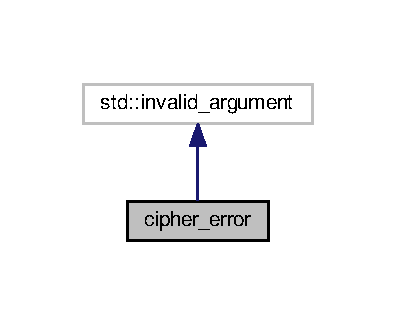
\includegraphics[width=190pt]{classcipher__error__inherit__graph}
\end{center}
\end{figure}


Граф связей класса cipher\+\_\+error\+:
\nopagebreak
\begin{figure}[H]
\begin{center}
\leavevmode
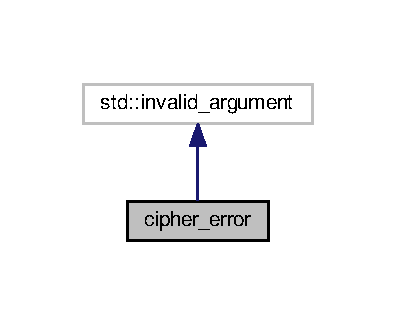
\includegraphics[width=190pt]{classcipher__error__coll__graph}
\end{center}
\end{figure}
\subsection*{Открытые члены}
\begin{DoxyCompactItemize}
\item 
\mbox{\Hypertarget{classcipher__error_aac662e216a84bfeb873303c7b88d029e}\label{classcipher__error_aac662e216a84bfeb873303c7b88d029e}} 
{\bfseries cipher\+\_\+error} (const std\+::string \&what\+\_\+arg)
\item 
\mbox{\Hypertarget{classcipher__error_a18cf27d9c2cd2538d3cb8f17e9a55f3e}\label{classcipher__error_a18cf27d9c2cd2538d3cb8f17e9a55f3e}} 
{\bfseries cipher\+\_\+error} (const char $\ast$what\+\_\+arg)
\end{DoxyCompactItemize}


\subsection{Подробное описание}
Класс-\/исключение. 

Призводный от класса invalid\+\_\+argument. При перегрузке конструкторов явно указаны вызов конструктора базового класса с параметром. 

Объявления и описания членов класса находятся в файле\+:\begin{DoxyCompactItemize}
\item 
\hyperlink{modAlphaCipher_8h}{mod\+Alpha\+Cipher.\+h}\end{DoxyCompactItemize}

\hypertarget{classmodAlphaCipher}{}\section{Класс mod\+Alpha\+Cipher}
\label{classmodAlphaCipher}\index{mod\+Alpha\+Cipher@{mod\+Alpha\+Cipher}}


Шифрование методом Гронсфельда  




{\ttfamily \#include $<$mod\+Alpha\+Cipher.\+h$>$}

\subsection*{Открытые члены}
\begin{DoxyCompactItemize}
\item 
\hyperlink{classmodAlphaCipher_a4f0a86c20f5d836f66cb1e640d875e6b}{mod\+Alpha\+Cipher} ()=delete
\begin{DoxyCompactList}\small\item\em Конструктор без параметров \end{DoxyCompactList}\item 
\hyperlink{classmodAlphaCipher_a76a420025b3c08f72c9b996d83c6ff09}{mod\+Alpha\+Cipher} (const std\+::string \&skey)
\begin{DoxyCompactList}\small\item\em Конструктор для установки ключа \end{DoxyCompactList}\item 
std\+::string \hyperlink{classmodAlphaCipher_ab855d6b2ba63a70d84abc8b15700da63}{encrypt} (const std\+::string \&open\+\_\+text)
\begin{DoxyCompactList}\small\item\em Зашифровывание \end{DoxyCompactList}\item 
std\+::string \hyperlink{classmodAlphaCipher_af1f0fa8ec93df56aa7657494de2a3f00}{decrypt} (const std\+::string \&cipher\+\_\+text)
\begin{DoxyCompactList}\small\item\em Расшифровывание \end{DoxyCompactList}\item 
std\+::wstring \hyperlink{classmodAlphaCipher_ad8496ce022685d8262b1f26f4b993de3}{towstr} (const std\+::string \&s)
\begin{DoxyCompactList}\small\item\em Перевод из кодировки U\+T\+F-\/8 в U\+T\+F-\/32. \end{DoxyCompactList}\item 
std\+::string \hyperlink{classmodAlphaCipher_aa0319b273a77c5ac7ea5407e7534e1c6}{fromwstr} (const std\+::wstring \&ws)
\begin{DoxyCompactList}\small\item\em Перевод из кодировки U\+T\+F-\/32 в U\+T\+F-\/8. \end{DoxyCompactList}\end{DoxyCompactItemize}


\subsection{Подробное описание}
Шифрование методом Гронсфельда 

Ключ устанавливается в конструкторе.\+Для зашифровывания и расшифровывания предназначены методы encrypt и decrypt. \begin{DoxyWarning}{Предупреждения}
Реализация только для русского языка 
\end{DoxyWarning}


\subsection{Конструктор(ы)}
\mbox{\Hypertarget{classmodAlphaCipher_a4f0a86c20f5d836f66cb1e640d875e6b}\label{classmodAlphaCipher_a4f0a86c20f5d836f66cb1e640d875e6b}} 
\index{mod\+Alpha\+Cipher@{mod\+Alpha\+Cipher}!mod\+Alpha\+Cipher@{mod\+Alpha\+Cipher}}
\index{mod\+Alpha\+Cipher@{mod\+Alpha\+Cipher}!mod\+Alpha\+Cipher@{mod\+Alpha\+Cipher}}
\subsubsection{\texorpdfstring{mod\+Alpha\+Cipher()}{modAlphaCipher()}\hspace{0.1cm}{\footnotesize\ttfamily [1/2]}}
{\footnotesize\ttfamily mod\+Alpha\+Cipher\+::mod\+Alpha\+Cipher (\begin{DoxyParamCaption}{ }\end{DoxyParamCaption})\hspace{0.3cm}{\ttfamily [delete]}}



Конструктор без параметров 

Запрещен \mbox{\Hypertarget{classmodAlphaCipher_a76a420025b3c08f72c9b996d83c6ff09}\label{classmodAlphaCipher_a76a420025b3c08f72c9b996d83c6ff09}} 
\index{mod\+Alpha\+Cipher@{mod\+Alpha\+Cipher}!mod\+Alpha\+Cipher@{mod\+Alpha\+Cipher}}
\index{mod\+Alpha\+Cipher@{mod\+Alpha\+Cipher}!mod\+Alpha\+Cipher@{mod\+Alpha\+Cipher}}
\subsubsection{\texorpdfstring{mod\+Alpha\+Cipher()}{modAlphaCipher()}\hspace{0.1cm}{\footnotesize\ttfamily [2/2]}}
{\footnotesize\ttfamily mod\+Alpha\+Cipher\+::mod\+Alpha\+Cipher (\begin{DoxyParamCaption}\item[{const std\+::string \&}]{skey }\end{DoxyParamCaption})}



Конструктор для установки ключа 

Перевод из кодировки U\+T\+F-\/32 в U\+T\+F-\/8.

Ключ проверяется на валидность. Переводится в кодировку U\+T\+F-\/32. Формируется вектор-\/ключ. 
\begin{DoxyParams}[1]{Аргументы}
\mbox{\tt in}  & {\em skey} & Ключ в кодировке U\+T\+F-\/8 \\
\hline
\end{DoxyParams}

\begin{DoxyExceptions}{Исключения}
{\em \hyperlink{classcipher__error}{cipher\+\_\+error}} & ключ вырожденный\\
\hline
\end{DoxyExceptions}

\begin{DoxyParams}[1]{Аргументы}
\mbox{\tt in}  & {\em s} & Строка в кодировке U\+T\+F-\/32 \\
\hline
\end{DoxyParams}
\begin{DoxyReturn}{Возвращает}
Строка в кодировке U\+T\+F-\/8 
\end{DoxyReturn}


\subsection{Методы}
\mbox{\Hypertarget{classmodAlphaCipher_af1f0fa8ec93df56aa7657494de2a3f00}\label{classmodAlphaCipher_af1f0fa8ec93df56aa7657494de2a3f00}} 
\index{mod\+Alpha\+Cipher@{mod\+Alpha\+Cipher}!decrypt@{decrypt}}
\index{decrypt@{decrypt}!mod\+Alpha\+Cipher@{mod\+Alpha\+Cipher}}
\subsubsection{\texorpdfstring{decrypt()}{decrypt()}}
{\footnotesize\ttfamily std\+::string mod\+Alpha\+Cipher\+::decrypt (\begin{DoxyParamCaption}\item[{const std\+::string \&}]{cipher\+\_\+text }\end{DoxyParamCaption})}



Расшифровывание 


\begin{DoxyParams}[1]{Аргументы}
\mbox{\tt in}  & {\em cipher\+\_\+text} & Зашифрованный текст в кодировке U\+T\+F-\/8. Не должен быть пустой строкой. Не должен содержать строчные символы и не-\/буквы. \\
\hline
\end{DoxyParams}
\begin{DoxyReturn}{Возвращает}
Расифрованная строка в кодировке U\+T\+F-\/8 
\end{DoxyReturn}

\begin{DoxyExceptions}{Исключения}
{\em \hyperlink{classcipher__error}{cipher\+\_\+error}} & текст пустой\\
\hline
\end{DoxyExceptions}

\begin{DoxyParams}[1]{Аргументы}
\mbox{\tt in}  & {\em cipher\+\_\+text} & Зашифрованный текст в кодировке U\+T\+F-\/8. Не должен быть пустой строкой. Не должен содержать строчные символы и небуквы. \\
\hline
\end{DoxyParams}
\begin{DoxyReturn}{Возвращает}
Расифрованная строка в кодировке U\+T\+F-\/8 
\end{DoxyReturn}

\begin{DoxyExceptions}{Исключения}
{\em \hyperlink{classcipher__error}{cipher\+\_\+error}} & текст пустой \\
\hline
\end{DoxyExceptions}
\mbox{\Hypertarget{classmodAlphaCipher_ab855d6b2ba63a70d84abc8b15700da63}\label{classmodAlphaCipher_ab855d6b2ba63a70d84abc8b15700da63}} 
\index{mod\+Alpha\+Cipher@{mod\+Alpha\+Cipher}!encrypt@{encrypt}}
\index{encrypt@{encrypt}!mod\+Alpha\+Cipher@{mod\+Alpha\+Cipher}}
\subsubsection{\texorpdfstring{encrypt()}{encrypt()}}
{\footnotesize\ttfamily std\+::string mod\+Alpha\+Cipher\+::encrypt (\begin{DoxyParamCaption}\item[{const std\+::string \&}]{open\+\_\+text }\end{DoxyParamCaption})}



Зашифровывание 


\begin{DoxyParams}[1]{Аргументы}
\mbox{\tt in}  & {\em open\+\_\+text} & Открытый текст в кодировке U\+T\+F-\/8. Не должен быть пустой строкой. Строчные символы автоматически преобразуются к прописным.\+Все не-\/буквы удаляются. \\
\hline
\end{DoxyParams}
\begin{DoxyReturn}{Возвращает}
Зашифрованная строка в кодировке U\+T\+F-\/8 
\end{DoxyReturn}

\begin{DoxyExceptions}{Исключения}
{\em \hyperlink{classcipher__error}{cipher\+\_\+error}} & текст пустой\\
\hline
\end{DoxyExceptions}
11$\ast$ 
\begin{DoxyParams}[1]{Аргументы}
\mbox{\tt in}  & {\em open\+\_\+text} & Открытый текст. Не должен быть пустой строкой. Строчные символы автоматически преобразуются к прописным. Все не-\/буквы удаляются \\
\hline
\end{DoxyParams}
\begin{DoxyReturn}{Возвращает}
Зашифрованная строка 
\end{DoxyReturn}

\begin{DoxyExceptions}{Исключения}
{\em \hyperlink{classcipher__error}{cipher\+\_\+error},если} & текст пустой \\
\hline
\end{DoxyExceptions}
\mbox{\Hypertarget{classmodAlphaCipher_aa0319b273a77c5ac7ea5407e7534e1c6}\label{classmodAlphaCipher_aa0319b273a77c5ac7ea5407e7534e1c6}} 
\index{mod\+Alpha\+Cipher@{mod\+Alpha\+Cipher}!fromwstr@{fromwstr}}
\index{fromwstr@{fromwstr}!mod\+Alpha\+Cipher@{mod\+Alpha\+Cipher}}
\subsubsection{\texorpdfstring{fromwstr()}{fromwstr()}}
{\footnotesize\ttfamily std\+::string mod\+Alpha\+Cipher\+::fromwstr (\begin{DoxyParamCaption}\item[{const std\+::wstring \&}]{ws }\end{DoxyParamCaption})}



Перевод из кодировки U\+T\+F-\/32 в U\+T\+F-\/8. 


\begin{DoxyParams}[1]{Аргументы}
\mbox{\tt in}  & {\em s} & Строка в кодировке U\+T\+F-\/32 \\
\hline
\end{DoxyParams}
\begin{DoxyReturn}{Возвращает}
Строка в кодировке U\+T\+F-\/8 
\end{DoxyReturn}
\mbox{\Hypertarget{classmodAlphaCipher_ad8496ce022685d8262b1f26f4b993de3}\label{classmodAlphaCipher_ad8496ce022685d8262b1f26f4b993de3}} 
\index{mod\+Alpha\+Cipher@{mod\+Alpha\+Cipher}!towstr@{towstr}}
\index{towstr@{towstr}!mod\+Alpha\+Cipher@{mod\+Alpha\+Cipher}}
\subsubsection{\texorpdfstring{towstr()}{towstr()}}
{\footnotesize\ttfamily std\+::wstring mod\+Alpha\+Cipher\+::towstr (\begin{DoxyParamCaption}\item[{const std\+::string \&}]{s }\end{DoxyParamCaption})}



Перевод из кодировки U\+T\+F-\/8 в U\+T\+F-\/32. 


\begin{DoxyParams}[1]{Аргументы}
\mbox{\tt in}  & {\em s} & Строка в кодировке U\+T\+F-\/8 \\
\hline
\end{DoxyParams}
\begin{DoxyReturn}{Возвращает}
Строка в кодировке U\+T\+F-\/32 
\end{DoxyReturn}


Объявления и описания членов классов находятся в файлах\+:\begin{DoxyCompactItemize}
\item 
\hyperlink{modAlphaCipher_8h}{mod\+Alpha\+Cipher.\+h}\item 
\hyperlink{modAlphaCipher_8cpp}{mod\+Alpha\+Cipher.\+cpp}\end{DoxyCompactItemize}

\chapter{Файлы}
\hypertarget{main_8cpp}{}\section{Файл main.\+cpp}
\label{main_8cpp}\index{main.\+cpp@{main.\+cpp}}


Заголовочный файл для модуля \hyperlink{main_8cpp}{main.\+cpp}.  


{\ttfamily \#include $<$iostream$>$}\newline
{\ttfamily \#include $<$cctype$>$}\newline
{\ttfamily \#include $<$codecvt$>$}\newline
{\ttfamily \#include $<$locale$>$}\newline
{\ttfamily \#include \char`\"{}mod\+Alpha\+Cipher.\+h\char`\"{}}\newline
Граф включаемых заголовочных файлов для main.\+cpp\+:
\nopagebreak
\begin{figure}[H]
\begin{center}
\leavevmode
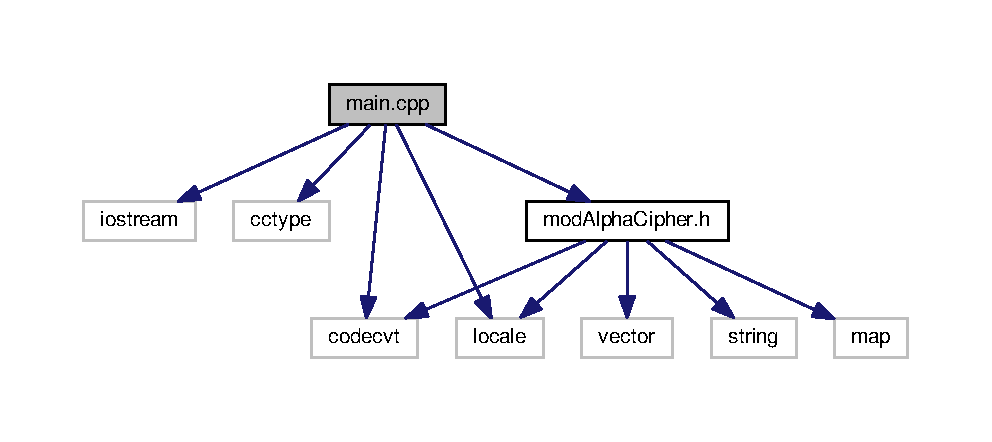
\includegraphics[width=350pt]{main_8cpp__incl}
\end{center}
\end{figure}
\subsection*{Функции}
\begin{DoxyCompactItemize}
\item 
\mbox{\Hypertarget{main_8cpp_a3eacb83174d2a9fbf9b313ebf1a9a883}\label{main_8cpp_a3eacb83174d2a9fbf9b313ebf1a9a883}} 
bool {\bfseries is\+Valid} (const string \&s)
\item 
int \hyperlink{main_8cpp_a3c04138a5bfe5d72780bb7e82a18e627}{main} (int argc, char $\ast$$\ast$argv)
\begin{DoxyCompactList}\small\item\em Интерфейс программы \end{DoxyCompactList}\end{DoxyCompactItemize}


\subsection{Подробное описание}
Заголовочный файл для модуля \hyperlink{main_8cpp}{main.\+cpp}. 

\begin{DoxyAuthor}{Автор}
Максимов О.\+В. 
\end{DoxyAuthor}
\begin{DoxyVersion}{Версия}
1.\+0.\+0 
\end{DoxyVersion}
\begin{DoxyDate}{Дата}
13.\+06.\+2019 
\end{DoxyDate}


\subsection{Функции}
\mbox{\Hypertarget{main_8cpp_a3c04138a5bfe5d72780bb7e82a18e627}\label{main_8cpp_a3c04138a5bfe5d72780bb7e82a18e627}} 
\index{main.\+cpp@{main.\+cpp}!main@{main}}
\index{main@{main}!main.\+cpp@{main.\+cpp}}
\subsubsection{\texorpdfstring{main()}{main()}}
{\footnotesize\ttfamily int main (\begin{DoxyParamCaption}\item[{int}]{argc,  }\item[{char $\ast$$\ast$}]{argv }\end{DoxyParamCaption})}



Интерфейс программы 

Осуществелние выбора ключа и операции 0, 1 или 2. В зависимости от выбора выполняются следующие действия\+: выход, зашифровка, расшифровка. ввод ключа

ввод числа 
\hypertarget{modAlphaCipher_8cpp}{}\section{Файл mod\+Alpha\+Cipher.\+cpp}
\label{modAlphaCipher_8cpp}\index{mod\+Alpha\+Cipher.\+cpp@{mod\+Alpha\+Cipher.\+cpp}}


Заголовочный файл для модуля \hyperlink{modAlphaCipher_8cpp}{mod\+Alpha\+Cipher.\+cpp}.  


{\ttfamily \#include \char`\"{}mod\+Alpha\+Cipher.\+h\char`\"{}}\newline
Граф включаемых заголовочных файлов для mod\+Alpha\+Cipher.\+cpp\+:
\nopagebreak
\begin{figure}[H]
\begin{center}
\leavevmode
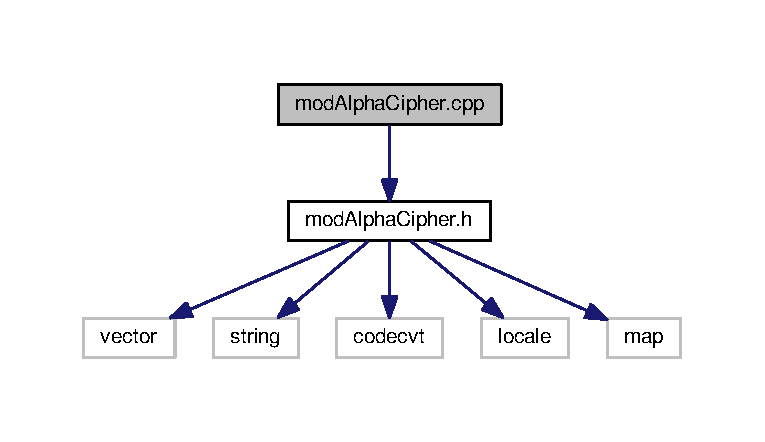
\includegraphics[width=350pt]{modAlphaCipher_8cpp__incl}
\end{center}
\end{figure}


\subsection{Подробное описание}
Заголовочный файл для модуля \hyperlink{modAlphaCipher_8cpp}{mod\+Alpha\+Cipher.\+cpp}. 

\begin{DoxyAuthor}{Автор}
Максимов О.\+В. 
\end{DoxyAuthor}
\begin{DoxyVersion}{Версия}
1.\+0.\+0 
\end{DoxyVersion}
\begin{DoxyDate}{Дата}
13.\+06.\+2019 
\end{DoxyDate}

\hypertarget{modAlphaCipher_8h}{}\section{Файл mod\+Alpha\+Cipher.\+h}
\label{modAlphaCipher_8h}\index{mod\+Alpha\+Cipher.\+h@{mod\+Alpha\+Cipher.\+h}}


Заголовочный файл для модуля Gronsfeld.  


{\ttfamily \#include $<$vector$>$}\newline
{\ttfamily \#include $<$string$>$}\newline
{\ttfamily \#include $<$codecvt$>$}\newline
{\ttfamily \#include $<$locale$>$}\newline
{\ttfamily \#include $<$map$>$}\newline
Граф включаемых заголовочных файлов для mod\+Alpha\+Cipher.\+h\+:
\nopagebreak
\begin{figure}[H]
\begin{center}
\leavevmode
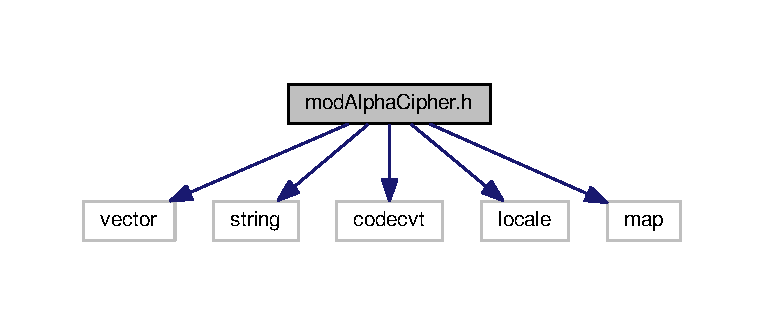
\includegraphics[width=350pt]{modAlphaCipher_8h__incl}
\end{center}
\end{figure}
Граф файлов, в которые включается этот файл\+:
\nopagebreak
\begin{figure}[H]
\begin{center}
\leavevmode
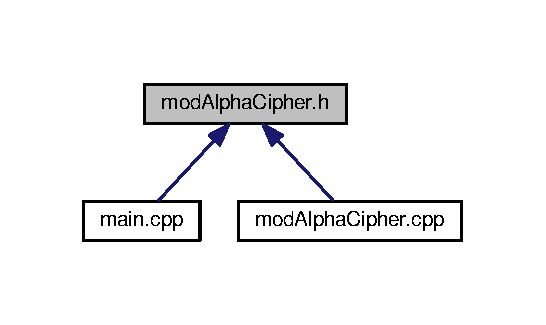
\includegraphics[width=262pt]{modAlphaCipher_8h__dep__incl}
\end{center}
\end{figure}
\subsection*{Классы}
\begin{DoxyCompactItemize}
\item 
class \hyperlink{classmodAlphaCipher}{mod\+Alpha\+Cipher}
\begin{DoxyCompactList}\small\item\em Шифрование методом Гронсфельда \end{DoxyCompactList}\item 
class \hyperlink{classcipher__error}{cipher\+\_\+error}
\begin{DoxyCompactList}\small\item\em Класс-\/исключение. \end{DoxyCompactList}\end{DoxyCompactItemize}


\subsection{Подробное описание}
Заголовочный файл для модуля Gronsfeld. 

\begin{DoxyAuthor}{Автор}
Максимов О.\+В. 
\end{DoxyAuthor}
\begin{DoxyVersion}{Версия}
1.\+0.\+0 
\end{DoxyVersion}
\begin{DoxyDate}{Дата}
13.\+06.\+2019 
\end{DoxyDate}

%--- End generated contents ---

% Index
\backmatter
\newpage
\phantomsection
\clearemptydoublepage
\addcontentsline{toc}{chapter}{Алфавитный указатель}
\printindex

\end{document}
